\documentclass[numbers=noenddot, 12pt, a4paper, oneside]{scrbook}
\usepackage{blindtext}
\usepackage[utf8]{inputenc}
\usepackage{float}
\usepackage{tabularx}
\usepackage{graphicx}
\def\Plus{\texttt{+}}
\usepackage{listings}
\usepackage{color}

\definecolor{dkgreen}{rgb}{0,0.6,0}
\definecolor{gray}{rgb}{0.5,0.5,0.5}
\definecolor{mauve}{rgb}{0.58,0,0.82}

\usepackage{xcolor}
\usepackage{listings}
\definecolor{mGreen}{rgb}{0,0.6,0}
\definecolor{mGray}{rgb}{0.5,0.5,0.5}
\definecolor{mPurple}{rgb}{0.58,0,0.82}
\definecolor{backgroundColour}{rgb}{0.95,0.95,0.92}

\lstset{frame=tb,
	language=Java,
	aboveskip=3mm,
	belowskip=3mm,
	showstringspaces=false,
	columns=flexible,
	basicstyle={\small\ttfamily},
	numbers=none,
	numberstyle=\tiny\color{gray},
	keywordstyle=\color{blue},
	commentstyle=\color{dkgreen},
	stringstyle=\color{mauve},
	breaklines=false,
	breakatwhitespace=true,
	tabsize=3
}

\lstdefinestyle{CStyle}{
	backgroundcolor=\color{backgroundColour},   
	commentstyle=\color{mGreen},
	keywordstyle=\color{magenta},
	numberstyle=\tiny\color{mGray},
	stringstyle=\color{mPurple},
	basicstyle=\footnotesize,
	breakatwhitespace=false,         
	breaklines=true,                 
	captionpos=b,                    
	keepspaces=true,                 
	numbers=left,                    
	numbersep=5pt,                  
	showspaces=false,                
	showstringspaces=false,
	showtabs=false,                  
	tabsize=2,
	language=C
}


\begin{document}

\begin{titlepage}
	\centering
	{\scshape\LARGE Politecnico di Milano \par}
	\vspace{1cm}
	
\includegraphics[width=0.35\textwidth]{polimi-logo}\par
	\vspace{1cm}

	{\scshape\Large Design and Implementation of Mobile Applications\par}
	\vspace{1.5cm}
	{\huge\bfseries iSport \par}
	\vspace{1cm}
	{\Large\bfseries Design Document \par}
	\vspace{3cm}
	{\Large\itshape di\par}
	{\Large\itshape Gianluigi Oliva\par}
	\vspace{1.5cm}
	\vfill
	


	\vfill

	% Bottom of the page
	{\large \today\par}
\end{titlepage}

\newpage
\tableofcontents
\newpage


\chapter{Introduction}

\section{Purpose}
The purpose of this document is to describe the design and prototyping phases used for the realization of the “iSport” mobile application. In detail, the main components, features and user experience will be discussed.

The main aim of iSport application is visualizing information and data related to the sport field. In particular, we will focus on the most relevant daily news, also showing a section with all football final scores. Inoltre per favorire la creazione di una comunità di discussione l'applicazione fornirà un sistema di live chat attraverso cui scambiarsi pareri.

This project is the result of the  implementation of the knowledge acquired during the course ”Design and Implementation of Mobile Applications” provided by the Milan Polytechnic.

\section{Intended Audience}
This document is produced for those who develop, evaluate and use iSport mobile application:
\begin{itemize}
	\item The engineers who had the idea and developed the application.
	\item The testers that must verify the effective implementation of all the described components and functions.
	\item The user who will use the application and take advantage of its functionalities.
	\item The future contributors who wish to develop new features.
\end{itemize}

\section{Definitions, acronyms, abbreviations}
\subsection*{Definitions}
\begin{itemize}
	\item \textbf{Platform}: The application as a whole.
	\item \textbf{Guest}: A person who can view public contents
	\item \textbf{User}: A guest who already performed the login operation successfully.
	\item \textbf{Match}: A match between two teams that has already occurred or is in progress
	\item \textbf{Framework}: Reusable set of libraries or classes for a software system.
	\item \textbf{News}: A news related to the world of sport present in some journalism
	\item \textbf{Forecast}: A prediction on the football scores among a class of possible results
	\item \textbf{Odds}: The remuneration value of a prediction relative to a given match
	\item \textbf{REST}: is a way of providing interoperability between computer systems on the Internet.
\end{itemize}
\subsection*{Acronyms}
\begin{itemize}
	\item \textbf{MVC}: Model - View - Controller
	\item \textbf{HTTPS}: HyperText Transfer Protocol Secure
	\item \textbf{IDE}: Integrated Development Environment
	\item \textbf{API}: Application Programming Interface
	\item \textbf{JSON}: JavaScript Object Notation
	\item \textbf{UML}: Unified Modelling Language.
	\item \textbf{UX}: User Experience
	\item \textbf{URL}: Uniform Resource Locator
\end{itemize}
\subsection*{Abbreviations}
\begin{itemize}
	\item \textbf{App}: Mobile Application 
\end{itemize}

\section{Mobile Application Scope}
iSport has been developed for those who love sports, with the aim to unify under one application all the services on the market. In this way we want to give an ongoing service to the end user, without having to browse multiple applications to achieve the same result.\\
In particular, the application will be divided into three screens:
\begin{itemize}
	\item \textbf{News}
	\item \textbf{Live}
	\item \textbf{Bet}
	\item \textbf{Chat}
\end{itemize}
In the ”News” section there will be the daily sport news displayed with a preview image and a small description. Moreover, by pressing on the single news you can read the complete article.\\
In the ”Live” section there will be all current matches with the final scores if already completed or the current one if still in progress. Pressing on the single game, the user will consult all the related information such as the markers and goal time, cards, training and statistics.\\
In the ”Bet” section there will be the shares related to the daily football matches. By pressing on the single one the user will bet on the winning game composing a ticket; once the process is completed the application will calculate the potential winnings based the bet amount.\\
Nella sezione "Chat" ci si collegherà ad una room globale in cui poter parlare con altri utenti che stanno utilizzando l'applicazione per scambiarsi commenti e pareri.


\section{Framework}
The development of iSport was achieved through the use of native iOS SDKs, in particular by using the Swift programming language. This choice allowed greater control of system resources and access to system services, otherwise not possible if using cross-platform frameworks such as PhoneGap or React Native. The purpose is to implement different functionalities and integration with other sites.

\section{Functional Requirements}
The product provides to users a simple and user-friendly interface to:
\begin{itemize}
	\item View news previews
	\item Read the complete article
	\item View football match results real time
	\item Display goal-scores
	\item Display booking (caution)
	\item Display team playing the match
	\item Display statistics
	\item Display game share 
	\item Compose your ticket
	\item Display the potential winnings of the ticket
	\item Condividere delle notizie su Facebook
	\item Salvare delle notizie tra i preferiti
	\item Chattare con altri utenti
	\item Esegure l'accesso
\end{itemize}
\section{Non Functional Requirements}
The application must be able to:
\begin{itemize}
	\item Run both on phone and tablet (only if they have an iOS).
	\item Work without requiring user sensitive data and services that may require a user cost (such as calls or SMS).
	\item Occupy the entire screen available.
	\item Keep preferences and status at every start.
\end{itemize}

\section{Assumptions, Dependencies and Constraints\\}

\subsection*{Costraints}

\begin{itemize}
	\item \textbf{Hardware limitations}: our application runs on every mobile device like smartphones and tablets. Therefore, as the App consumes a low amount of RAM, the only hardware constraint for the users is to have a mid-range device. (for instance iPhone 5 or better).
	\item \textbf{Parallel operations}: the application must be able to handle multiple parallel requests with high reactivity.
\end{itemize}

\subsection*{Assumptions and Dependecies}
\begin{itemize}
	\item \textbf{Internet Connection}: the device used by the users dispose of an internet connection and a sufficient bandwidth to use the application.
	\item \textbf{No privileged users}: there are no priviled users or administrators with particular functions.
	\item \textbf{No user connections}: every user is independent from the others.
	\item \textbf{API availability}: the API provided by third part's services are always available.
	\item \textbf{OS Permission Granted}: the user will always grant to his OS's device the permission to access to all the needed services.
\end{itemize}


\chapter{Architecture}
\section{Database}
Since the application receives all the necessary data from external services through the API, the only data that need to be saved are the games that make up a ticket. Moreover, since there is no interaction between the different users, the data is saved locally using the Core Data present in the iOS SDK.
\begin{figure}[H]
	\centering
	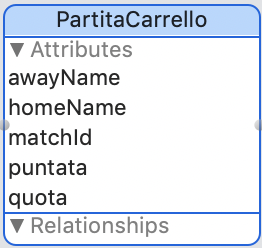
\includegraphics[width=0.2\textwidth]{images/DatiSchedina}
	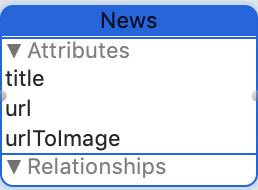
\includegraphics[width=0.2\textwidth]{images/DatiNews}
\end{figure}
Per permettere l'acquisto di schedine è stato usato un Database online utilizzando la piattaforma di Firebase. Il modello E/R utilizzato per quest'ultimo è il seguente:
\begin{figure}[H]
	\centering
	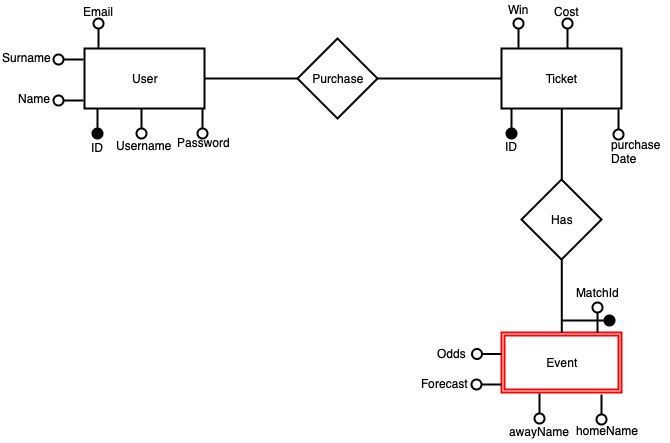
\includegraphics[width=0.7\textwidth]{images/ER.png}
\end{figure}
\newpage
Per garantire la privacy di ogni utente, l'accesso al Database è regolato mediante le seguenti rules:
\begin{lstlisting}[style=CStyle]
{
	"rules": {
		"Schedina": {
			"$uid": {
				".read": "$uid === auth.uid",
				".write": "$uid === auth.uid"
			}
		}
	}
}
\end{lstlisting}


\section{Client}
For the implementation of the application we have chosen a mobile back-end, that is a client architecture.  This choice was made mainly because the application does not interface with other users and because for various services it uses third-party APIs. Communication with third-party services is based on HTTPS REST requests, in particular through GET requests.\\
The client uses the traditional MVC pattern:
\begin{itemize}
	\item Model: this package contains all the classes representing data to be shown to the single user, taken by the Controller and published by the View.
	\item View: this package contains all the components that display data to the user and interact with him.
	\item Controller: this package contains all the objects in charge to interact between one or more view objects of the application and one or more model objects.
\end{itemize}

\chapter{Use case functional requirements analysis}
This section describes how actors can interact with iSport in order to use all the features implemented in the app. The focus of this part is on the front-end and we show the operations that can be performed by the actors without taking care of the system architecture behind the app.
\begin{figure}[H]
	\centering
	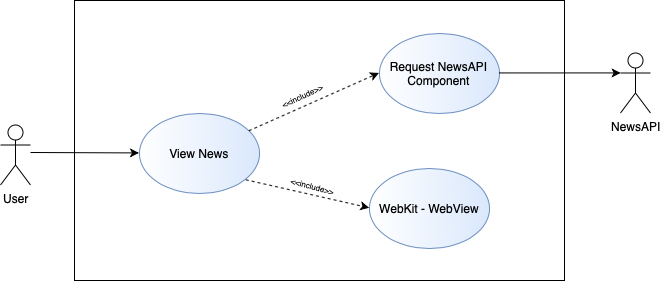
\includegraphics[width=0.7\textwidth]{images/ViewNews}
	\caption{Use case relativo alla visualizzazione e manipolazione delle notizie}
\end{figure}
\begin{figure}[H]
	\centering
	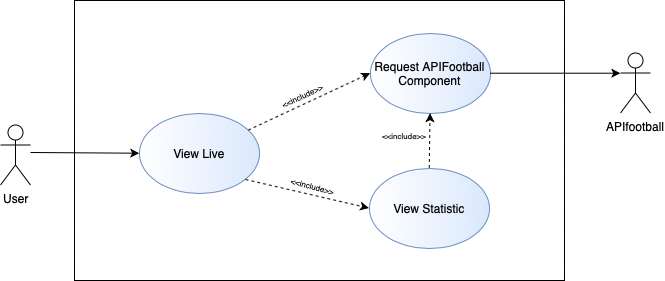
\includegraphics[width=0.7\textwidth]{images/ViewLive}
	\caption{Use case relativo alla visualizzazione e manipolazione dei risultati}
\end{figure}
\begin{figure}[H]
	\centering
	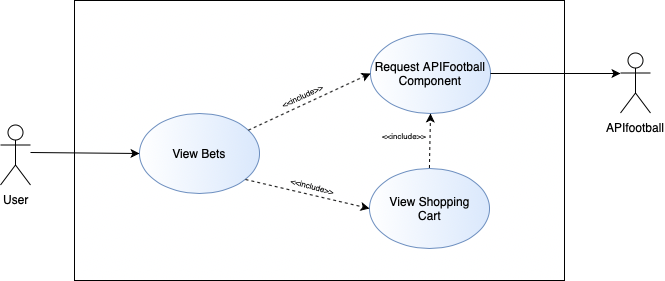
\includegraphics[width=0.7\textwidth]{images/ViewBet}
	\caption{Use case relativo alla visualizzazione e manipolazione delle quote}
\end{figure}
\begin{figure}[H]
	\centering
	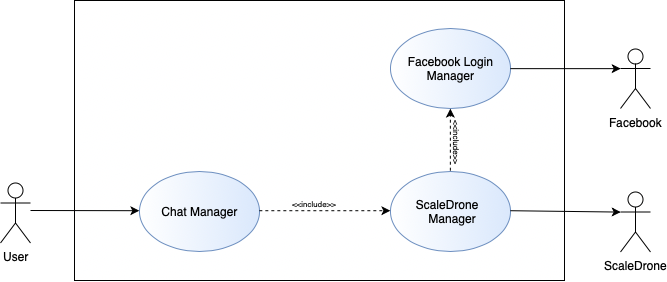
\includegraphics[width=0.7\textwidth]{images/Chat}
	\caption{Use case del servizio chat}
\end{figure}
\begin{figure}[H]
	\centering
	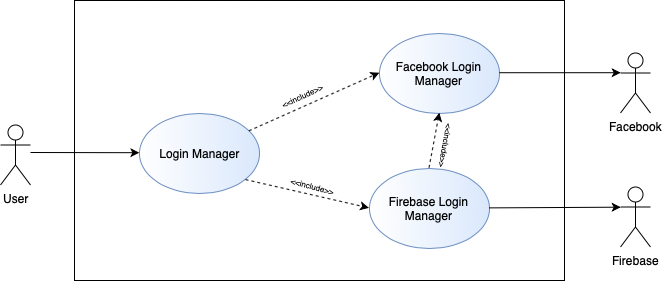
\includegraphics[width=0.7\textwidth]{images/Login}
	\caption{Use case per l'esecuzione del Login}
\end{figure}
\begin{figure}[H]
	\centering
	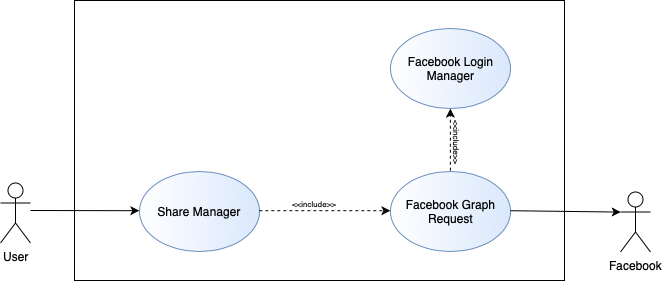
\includegraphics[width=0.7\textwidth]{images/Share}
	\caption{Use case relativo condivisione di notizie}
\end{figure}
\begin{figure}[H]
	\centering
	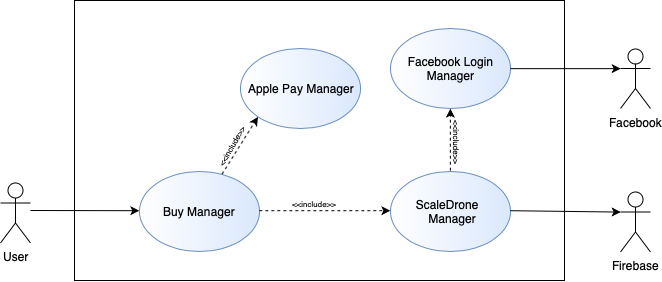
\includegraphics[width=0.7\textwidth]{images/Buy}
	\caption{Use case relativo all'acquisto di schedine}
\end{figure}
\subsection*{Login}
\begin{tabular}{|c|p{0.8\textwidth}|}
	\hline
	\parbox[c][6ex]{6ex}{\centering \textbf{Name}} & Login\\
	\hline
	\parbox[c][6ex]{6ex}{\centering \textbf{Actor}} & Guest \\
	\hline
	\parbox[c][10ex]{15ex}{\centering \textbf{Entry Condition}} & Guest with login credentials\\
	\hline
	\parbox[c][6ex]{15ex}{\centering \textbf{Goal}} &  1, 2\\
	\hline
	\parbox[c][10ex]{12ex}{\centering \textbf{Event Flow}} & \begin{itemize}
		\item L'utente apre l'applicazione
		\item L'utente preme sulla tab "Login" del "Side Menu"
		\item L'utente viene rimandato sul sito di Facebook per l'inserimento delle credenziali
		\item L'applicazione effettua il login tramite Facebook
		\item L'applicazione effettua il login a Firebase usando l'account di Facebook
	\end{itemize}\\
	\hline
	\parbox[c][7ex]{12ex}{\centering \textbf{Exit condition}} & Actor becomes User \\\hline
	\parbox[c][10ex]{13ex}{\centering \textbf{Exceptions}} & L'utente non è connesso alla rete. L'utente non ha un account Facebook. \\ \hline	
\end{tabular}
\newpage
\subsection*{Logout}
\begin{tabular}{|c|p{0.8\textwidth}|}
	\hline
	\parbox[c][6ex]{6ex}{\centering \textbf{Name}} & Logout\\
	\hline
	\parbox[c][6ex]{6ex}{\centering \textbf{Actor}} & User \\
	\hline
	\parbox[c][10ex]{15ex}{\centering \textbf{Entry Condition}} & Actor is logged in\\
	\hline
	\parbox[c][6ex]{15ex}{\centering \textbf{Goal}} &  1, 2\\
	\hline
	\parbox[c][10ex]{12ex}{\centering \textbf{Event Flow}} & \begin{itemize}
		\item L'utente preme sulla tab "Logout" del "Side Menu"
		\item L'applicazione effettua il logout da Facebook
		\item L'applicazione effettua il logout da Firebase
	\end{itemize}\\
	\hline
	\parbox[c][7ex]{12ex}{\centering \textbf{Exit condition}} & Actor is logged out and becomes Guest \\\hline
	\parbox[c][10ex]{13ex}{\centering \textbf{Exceptions}} & L'utente non è connesso alla rete. \\ \hline	
\end{tabular}
\newpage
\subsection*{Visualizzare Notizie}
\begin{tabular}{|c|p{0.8\textwidth}|}
	\hline
	\parbox[c][6ex]{6ex}{\centering \textbf{Name}} & Visualizzare Notizie\\
	\hline
	\parbox[c][6ex]{6ex}{\centering \textbf{Actor}} & Guest \\
	\hline
	\parbox[c][10ex]{15ex}{\centering \textbf{Entry Condition}} & L'attore ha scaricato l'applicazione\\
	\hline
	\parbox[c][6ex]{15ex}{\centering \textbf{Goal}} &  1, 2\\
	\hline
	\parbox[c][10ex]{12ex}{\centering \textbf{Event Flow}} & \begin{itemize}
		\item L'utente apre l'applicazione
		\item L'utente preme sulla tab "News" del "Side Menu"
		\item L'applicazione fornisce un elenco delle notizie principali
		\item L'utente preme sull'articolo di cui vuole visualizzare la notizia completa
		\item L'utente preme il tasto "Done" per terminare la lettura
	\end{itemize}\\
	\hline
	\parbox[c][7ex]{12ex}{\centering \textbf{Exit condition}} & L'utente ha letto la notizia di interesse. \\\hline
	\parbox[c][10ex]{13ex}{\centering \textbf{Exceptions}} & L'utente non è connesso alla rete e quindi non può inviare le richieste per ottenere gli articoli e quindi non può mostrarle. L'articolo è stato rimosso dal sito di origine, ma non nel database del servizio terzo \\ \hline	
\end{tabular}
\newpage
\subsection*{Condividere Notizie}
\begin{tabular}{|c|p{0.8\textwidth}|}
	\hline
	\parbox[c][6ex]{6ex}{\centering \textbf{Name}} & Condividere Notizie\\
	\hline
	\parbox[c][6ex]{6ex}{\centering \textbf{Actor}} & User \\
	\hline
	\parbox[c][10ex]{15ex}{\centering \textbf{Entry Condition}} & L'attore si è autenticato correttamente\\
	\hline
	\parbox[c][6ex]{15ex}{\centering \textbf{Goal}} &  1, 2\\
	\hline
	\parbox[c][10ex]{12ex}{\centering \textbf{Event Flow}} & \begin{itemize}
		\item L'utente apre l'applicazione
		\item L'utente preme sulla tab "News" del "Side Menu"
		\item L'applicazione fornisce un elenco delle notizie principali
		\item L'utente preme il simbolo di "Share" della notizia che vuole condividere
		\item L'utente compone l'eventuale messaggio da allegare nel post
		\item L'utente preme il tasto "Pubblica" per terminare la condivisione
	\end{itemize}\\
	\hline
	\parbox[c][7ex]{12ex}{\centering \textbf{Exit condition}} & L'utente ha condiviso su Facebook la notizia di interesse. \\\hline
	\parbox[c][10ex]{13ex}{\centering \textbf{Exceptions}} & L'utente non è connesso alla rete e quindi non può inviare le richieste per ottenere gli articoli e quindi non può mostrarle. L'articolo è stato rimosso dal sito di origine, ma non nel database del servizio terzo. La connessione è debole e l'applicazione non riesce a mandare i dati per la condivisione. \\ \hline	
\end{tabular}
\newpage
\subsection*{Salvare Notizie}
\begin{tabular}{|c|p{0.8\textwidth}|}
	\hline
	\parbox[c][6ex]{6ex}{\centering \textbf{Name}} & Salvare Notizie\\
	\hline
	\parbox[c][6ex]{6ex}{\centering \textbf{Actor}} & User \\
	\hline
	\parbox[c][10ex]{15ex}{\centering \textbf{Entry Condition}} & L'attore ha scaricato l'applicazione\\
	\hline
	\parbox[c][6ex]{15ex}{\centering \textbf{Goal}} &  1, 2\\
	\hline
	\parbox[c][10ex]{12ex}{\centering \textbf{Event Flow}} & \begin{itemize}
		\item L'utente apre l'applicazione
		\item L'utente preme sulla tab "News" del "Side Menu"
		\item L'applicazione fornisce un elenco delle notizie principali
		\item L'utente preme il simbolo di "Elenco" della notizia che vuole memorizzare
		\item L'applicazione memorizza le informazioni necessarie nel database locale
	\end{itemize}\\
	\hline
	\parbox[c][7ex]{12ex}{\centering \textbf{Exit condition}} & L'utente ha memorizzato una notizia per una visione successiva. \\\hline
	\parbox[c][10ex]{13ex}{\centering \textbf{Exceptions}} & L'utente non è connesso alla rete e quindi non può inviare le richieste per ottenere gli articoli e quindi non può mostrarle. L'articolo è stato rimosso dal sito di origine, ma non nel database del servizio terzo. \\ \hline	
\end{tabular}
\newpage
\subsection*{Visualizzare Notizie Salvate}
\begin{tabular}{|c|p{0.8\textwidth}|}
	\hline
	\parbox[c][6ex]{6ex}{\centering \textbf{Name}} & Visualizzare Notizie Salvate\\
	\hline
	\parbox[c][6ex]{6ex}{\centering \textbf{Actor}} & User \\
	\hline
	\parbox[c][10ex]{15ex}{\centering \textbf{Entry Condition}} & L'attore ha salvato delle notizie in precedenza\\
	\hline
	\parbox[c][6ex]{15ex}{\centering \textbf{Goal}} &  1, 2\\
	\hline
	\parbox[c][10ex]{12ex}{\centering \textbf{Event Flow}} & \begin{itemize}
		\item L'utente apre l'applicazione
		\item L'utente preme sulla tab "News" del "Side Menu"
		\item L'utente preme il tasto "Elenco" nella Navigation Bar per consultare le notizie salvate
		\item L'applicazione fornisce un elenco delle notizie salvate in precedenza
	\end{itemize}\\
	\hline
	\parbox[c][7ex]{12ex}{\centering \textbf{Exit condition}} & L'utente ha memorizzato una notizia per una visione successiva. \\\hline
	\parbox[c][10ex]{13ex}{\centering \textbf{Exceptions}} & L'utente non è connesso alla rete e quindi non può inviare le richieste per ottenere gli articoli e quindi non può mostrarle. L'articolo è stato rimosso dal sito di origine, ma non nel database del servizio terzo. \\ \hline	
\end{tabular}
\newpage
\subsection*{Visualizzare Partite}
\begin{tabular}{|c|p{0.8\textwidth}|}
	\hline
	\parbox[c][6ex]{6ex}{\centering \textbf{Name}} & Visualizzare Partite\\
	\hline
	\parbox[c][6ex]{6ex}{\centering \textbf{Actor}} & Guest \\
	\hline
	\parbox[c][10ex]{15ex}{\centering \textbf{Entry Condition}} & L'attore ha scaricato l'applicazione\\
	\hline
	\parbox[c][6ex]{15ex}{\centering \textbf{Goal}} &  3\\
	\hline
	\parbox[c][10ex]{12ex}{\centering \textbf{Event Flow}} & \begin{itemize}
		\item L'utente apre l'applicazione
		\item L'utente preme sulla tab "Live" del "Side Menu"
		\item L'applicazione fornisce un elenco delle partite del giorno
	\end{itemize}\\
	\hline
	\parbox[c][7ex]{12ex}{\centering \textbf{Exit condition}} & L'utente ha visualizzato i risultati delle partite. \\\hline
	\parbox[c][10ex]{13ex}{\centering \textbf{Exceptions}} & L'utente non è connesso alla rete e quindi non può inviare le richieste per ottenere i risultati e quindi non può mostrargli. La connessione potrebbe essere debole e quindi non riuscire a ricevere i dati richiesti. \\ \hline	
\end{tabular}



\newpage
\subsection*{Visualizzare Formazione Partita}
\begin{tabular}{|c|p{0.8\textwidth}|}
	\hline
	\parbox[c][6ex]{6ex}{\centering \textbf{Name}} & Visualizzare Formazione Partita\\
	\hline
	\parbox[c][6ex]{6ex}{\centering \textbf{Actor}} & Guest \\
	\hline
	\parbox[c][10ex]{15ex}{\centering \textbf{Entry Condition}} & L'attore ha scaricato l'applicazione\\
	\hline
	\parbox[c][6ex]{15ex}{\centering \textbf{Goal}} &  3, 6\\
	\hline
	\parbox[c][10ex]{12ex}{\centering \textbf{Event Flow}} & \begin{itemize}
		\item L'utente apre l'applicazione
		\item L'utente preme sulla tab "Live" del "Side Menu"
		\item L'applicazione fornisce un elenco delle partite del giorno
		\item L'utente preme sulla partita di cui vuole ottenere l'informazione richiesta
		\item L'utente preme sul bottone raffigurante il campo di gioco
	\end{itemize}\\
	\hline
	\parbox[c][7ex]{12ex}{\centering \textbf{Exit condition}} & L'utente ha visualizzato le formazioni delle due squadre della partita richiesta. \\\hline
	\parbox[c][10ex]{13ex}{\centering \textbf{Exceptions}} & L'utente non è connesso alla rete e quindi non può inviare le richieste per ottenere i risultati e quindi non può mostrargli. La connessione potrebbe essere debole e quindi non riuscire a ricevere i dati richiesti. \\ \hline	
\end{tabular}
\newpage
\subsection*{Visualizzare Marcatori Partita}
\begin{tabular}{|c|p{0.8\textwidth}|}
	\hline
	\parbox[c][6ex]{6ex}{\centering \textbf{Name}} & Visualizzare Marcatori Partita\\
	\hline
	\parbox[c][6ex]{6ex}{\centering \textbf{Actor}} & Guest \\
	\hline
	\parbox[c][10ex]{15ex}{\centering \textbf{Entry Condition}} & L'attore ha scaricato l'applicazione\\
	\hline
	\parbox[c][6ex]{15ex}{\centering \textbf{Goal}} &  3, 4\\
	\hline
	\parbox[c][10ex]{12ex}{\centering \textbf{Event Flow}} & \begin{itemize}
		\item L'utente apre l'applicazione
		\item L'utente preme sulla tab "Live" del "Side Menu"
		\item L'applicazione fornisce un elenco delle partite del giorno
		\item L'utente preme sulla partita di cui vuole ottenere l'informazione richiesta
		\item L'utente preme sul bottone raffigurante un pallore
	\end{itemize}\\
	\hline
	\parbox[c][7ex]{12ex}{\centering \textbf{Exit condition}} & L'utente ha visualizzato i marcatori della partita richiesta. \\\hline
	\parbox[c][10ex]{13ex}{\centering \textbf{Exceptions}} & L'utente non è connesso alla rete e quindi non può inviare le richieste per ottenere i risultati e quindi non può mostrargli. La connessione potrebbe essere debole e quindi non riuscire a ricevere i dati richiesti. \\ \hline	
\end{tabular}
\newpage
\subsection*{Visualizzare Statistiche Partita}
\begin{tabular}{|c|p{0.8\textwidth}|}
	\hline
	\parbox[c][6ex]{6ex}{\centering \textbf{Name}} & Visualizzare Statistiche Partita\\
	\hline
	\parbox[c][6ex]{6ex}{\centering \textbf{Actor}} & Guest \\
	\hline
	\parbox[c][10ex]{15ex}{\centering \textbf{Entry Condition}} & L'attore ha scaricato l'applicazione\\
	\hline
	\parbox[c][6ex]{15ex}{\centering \textbf{Goal}} &  3, 7\\
	\hline
	\parbox[c][10ex]{12ex}{\centering \textbf{Event Flow}} & \begin{itemize}
		\item L'utente apre l'applicazione
		\item L'utente preme sulla tab "Live" del "Side Menu"
		\item L'applicazione fornisce un elenco delle partite del giorno
		\item L'utente preme sulla partita di cui vuole ottenere l'informazione richiesta
		\item L'utente preme sul bottone raffigurante un grafico
	\end{itemize}\\
	\hline
	\parbox[c][7ex]{12ex}{\centering \textbf{Exit condition}} & L'utente ha visualizzato le statistiche della partita richiesta. \\\hline
	\parbox[c][10ex]{13ex}{\centering \textbf{Exceptions}} & L'utente non è connesso alla rete e quindi non può inviare le richieste per ottenere i risultati e quindi non può mostrargli. La connessione potrebbe essere debole e quindi non riuscire a ricevere i dati richiesti. \\ \hline	
\end{tabular}
\newpage
\subsection*{Visualizzare Ammonizioni Partita}
\begin{tabular}{|c|p{0.8\textwidth}|}
	\hline
	\parbox[c][6ex]{6ex}{\centering \textbf{Name}} & Visualizzare Ammonizioni Partita\\
	\hline
	\parbox[c][6ex]{6ex}{\centering \textbf{Actor}} & Guest \\
	\hline
	\parbox[c][10ex]{15ex}{\centering \textbf{Entry Condition}} & L'attore ha scaricato l'applicazione\\
	\hline
	\parbox[c][6ex]{15ex}{\centering \textbf{Goal}} &  3, 5\\
	\hline
	\parbox[c][10ex]{12ex}{\centering \textbf{Event Flow}} & \begin{itemize}
		\item L'utente apre l'applicazione
		\item L'utente preme sulla tab "Live" del "Side Menu"
		\item L'applicazione fornisce un elenco delle partite del giorno
		\item L'utente preme sulla partita di cui vuole ottenere l'informazione richiesta
		\item L'utente preme sul bottone raffigurante un cartellino
	\end{itemize}\\
	\hline
	\parbox[c][7ex]{12ex}{\centering \textbf{Exit condition}} & L'utente ha visualizzato gli ammoniti ed espulsi della partita richiesta. \\\hline
	\parbox[c][10ex]{13ex}{\centering \textbf{Exceptions}} & L'utente non è connesso alla rete e quindi non può inviare le richieste per ottenere i risultati e quindi non può mostrargli. La connessione potrebbe essere debole e quindi non riuscire a ricevere i dati richiesti. \\ \hline	
\end{tabular}
\newpage
\subsection*{Visualizzare Quote}
\begin{tabular}{|c|p{0.8\textwidth}|}
	\hline
	\parbox[c][6ex]{6ex}{\centering \textbf{Name}} & Visualizzare Quote\\
	\hline
	\parbox[c][6ex]{6ex}{\centering \textbf{Actor}} & Guest \\
	\hline
	\parbox[c][10ex]{15ex}{\centering \textbf{Entry Condition}} & L'attore ha scaricato l'applicazione\\
	\hline
	\parbox[c][6ex]{15ex}{\centering \textbf{Goal}} &  8\\
	\hline
	\parbox[c][10ex]{12ex}{\centering \textbf{Event Flow}} & \begin{itemize}
		\item L'utente apre l'applicazione
		\item L'utente preme sulla tab "Bet" del "Side Menu"
		\item L'applicazione fornisce un elenco delle quote dei principali pronostici delle partite odierne
	\end{itemize}\\
	\hline
	\parbox[c][7ex]{12ex}{\centering \textbf{Exit condition}} & L'utente ha visualizzatole quote delle partite odierne. \\\hline
	\parbox[c][10ex]{13ex}{\centering \textbf{Exceptions}} & L'utente non è connesso alla rete e quindi non può inviare le richieste per ottenere le quote. La connessione potrebbe essere debole e quindi non riuscire a ricevere i dati richiesti. \\ \hline	
\end{tabular}
\newpage
\subsection*{Visualizza Schedina Composta}
\begin{tabular}{|c|p{0.8\textwidth}|}
	\hline
	\parbox[c][6ex]{6ex}{\centering \textbf{Name}} & Visualizza Schedina Composta\\
	\hline
	\parbox[c][6ex]{6ex}{\centering \textbf{Actor}} & Guest \\
	\hline
	\parbox[c][10ex]{15ex}{\centering \textbf{Entry Condition}} & L'attore ha scaricato l'applicazione\\
	\hline
	\parbox[c][6ex]{15ex}{\centering \textbf{Goal}} &  9\\
	\hline
	\parbox[c][10ex]{12ex}{\centering \textbf{Event Flow}} & \begin{itemize}
		\item L'utente apre l'applicazione
		\item L'utente preme sulla tab "Bet" del "Side Menu"
		\item L'utente preme sul bottone raffigurante un carrello nella NavBar
	\end{itemize}\\
	\hline
	\parbox[c][7ex]{12ex}{\centering \textbf{Exit condition}} & L'utente visualizza i pronostici presenti nella schedina.\\\hline
	\parbox[c][10ex]{13ex}{\centering \textbf{Exceptions}} & L'utente non è connesso alla rete e quindi non può inviare le richieste per ottenere le quote. La connessione potrebbe essere debole e quindi non riuscire a ricevere i dati richiesti. \\ \hline	
\end{tabular}
\newpage
\subsection*{Aggiungere Partita a Schedina}
\begin{tabular}{|c|p{0.8\textwidth}|}
	\hline
	\parbox[c][6ex]{6ex}{\centering \textbf{Name}} & Aggiungere Partita a Schedina\\
	\hline
	\parbox[c][6ex]{6ex}{\centering \textbf{Actor}} & Guest \\
	\hline
	\parbox[c][10ex]{15ex}{\centering \textbf{Entry Condition}} & L'attore ha scaricato l'applicazione\\
	\hline
	\parbox[c][6ex]{15ex}{\centering \textbf{Goal}} &  9\\
	\hline
	\parbox[c][10ex]{12ex}{\centering \textbf{Event Flow}} & \begin{itemize}
		\item L'utente apre l'applicazione
		\item L'utente preme sulla tab "Bet" del "Side Menu"
		\item L'applicazione fornisce un elenco delle quote dei principali pronostici delle partite odierne
		\item L'utente preme sulla quota relativa al pronostico e partita da aggiungere
	\end{itemize}\\
	\hline
	\parbox[c][7ex]{12ex}{\centering \textbf{Exit condition}} & L'utente ha aggiunto un pronostico di una partita alla schedina.\\\hline
	\parbox[c][10ex]{13ex}{\centering \textbf{Exceptions}} & L'utente non è connesso alla rete e quindi non può inviare le richieste per ottenere le quote. La connessione potrebbe essere debole e quindi non riuscire a ricevere i dati richiesti. \\ \hline	
\end{tabular}
\newpage
\subsection*{Eliminare Partita da Schedina}
\begin{tabular}{|c|p{0.8\textwidth}|}
	\hline
	\parbox[c][6ex]{6ex}{\centering \textbf{Name}} & Eliminare Partita a Schedina\\
	\hline
	\parbox[c][6ex]{6ex}{\centering \textbf{Actor}} & Guest \\
	\hline
	\parbox[c][10ex]{15ex}{\centering \textbf{Entry Condition}} & L'attore ha scaricato l'applicazione\\
	\hline
	\parbox[c][6ex]{15ex}{\centering \textbf{Goal}} &  9\\
	\hline
	\parbox[c][10ex]{12ex}{\centering \textbf{Event Flow}} & \begin{itemize}
		\item L'utente apre l'applicazione
		\item L'utente preme sulla tab "Bet" del "Side Menu"
		\item L'utente preme sul bottone raffigurante un carrello nella NavBar
		\item L'utente effettua uno swipe verso sinistra sulla partita da eliminare
	\end{itemize}\\
	\hline
	\parbox[c][7ex]{12ex}{\centering \textbf{Exit condition}} & L'utente ha eliminato un pronostico di una partita alla schedina.\\\hline
	\parbox[c][10ex]{13ex}{\centering \textbf{Exceptions}} & Nessuna Eccezione\\ \hline	
\end{tabular}
\newpage
\subsection*{Calcolare potenziale Vincita Schedina}
\begin{tabular}{|c|p{0.8\textwidth}|}
	\hline
	\parbox[c][6ex]{6ex}{\centering \textbf{Name}} & Calcolare potenziale Vincita Schedina\\
	\hline
	\parbox[c][6ex]{6ex}{\centering \textbf{Actor}} & Guest \\
	\hline
	\parbox[c][10ex]{15ex}{\centering \textbf{Entry Condition}} & L'attore ha scaricato l'applicazione\\
	\hline
	\parbox[c][6ex]{15ex}{\centering \textbf{Goal}} &  10\\
	\hline
	\parbox[c][10ex]{12ex}{\centering \textbf{Event Flow}} & \begin{itemize}
		\item L'utente apre l'applicazione
		\item L'utente preme sulla tab "Bet" del "Side Menu"
		\item L'utente preme sul bottone raffigurante un carrello nella NavBar
		\item L'utente inserisce l'importo da giocare nell'apposito input
		\item L'utente preme il tasto "Done"
	\end{itemize}\\
	\hline
	\parbox[c][7ex]{12ex}{\centering \textbf{Exit condition}} & L'utente visualizza la potenziale vincita della schedina attuale.\\\hline
	\parbox[c][10ex]{13ex}{\centering \textbf{Exceptions}} & Nessuna Eccezione \\ \hline	
\end{tabular}
\newpage
\subsection*{Acquisto Schedina}
\begin{tabular}{|c|p{0.8\textwidth}|}
	\hline
	\parbox[c][6ex]{6ex}{\centering \textbf{Name}} & Acquisto Schedina\\
	\hline
	\parbox[c][6ex]{6ex}{\centering \textbf{Actor}} & User \\
	\hline
	\parbox[c][10ex]{15ex}{\centering \textbf{Entry Condition}} & L'attore si è autenticato correttamente\\
	\hline
	\parbox[c][6ex]{15ex}{\centering \textbf{Goal}} &  10\\
	\hline
	\parbox[c][10ex]{12ex}{\centering \textbf{Event Flow}} & \begin{itemize}
		\item L'utente apre l'applicazione
		\item L'utente preme sulla tab "Bet" del "Side Menu"
		\item L'utente preme sul bottone raffigurante un carrello nella NavBar
		\item L'utente inserisce l'importo che vuole giocare
		\item L'utente preme sul bottone "Buy"
	\end{itemize}\\
	\hline
	\parbox[c][7ex]{12ex}{\centering \textbf{Exit condition}} & L'utente acquista la schedina attuale.\\\hline
	\parbox[c][10ex]{13ex}{\centering \textbf{Exceptions}} & La connessione è assente e non può portare a termine l'acquisto. L'utente non è autenticato. L'utente non ha inserito nessuna partita nella schedina \\ \hline	
\end{tabular}
\newpage
\subsection*{Visualizza Schedine Acquistate}
\begin{tabular}{|c|p{0.8\textwidth}|}
	\hline
	\parbox[c][6ex]{6ex}{\centering \textbf{Name}} & Visualizza Schedine Acquistate\\
	\hline
	\parbox[c][6ex]{6ex}{\centering \textbf{Actor}} & User \\
	\hline
	\parbox[c][10ex]{15ex}{\centering \textbf{Entry Condition}} & L'attore si è autenticato correttamente\\
	\hline
	\parbox[c][6ex]{15ex}{\centering \textbf{Goal}} &  9\\
	\hline
	\parbox[c][10ex]{12ex}{\centering \textbf{Event Flow}} & \begin{itemize}
		\item L'utente apre l'applicazione
		\item L'utente preme sulla tab "Bet" del "Side Menu"
		\item L'utente preme sul bottone "cronologia" nella NavBar
		\item L'applicazione scarica le informazioni su tutte le schedine acquistate
		\item L'utente preme sulla cella corrispondente alla schedina che vuole visualizzare
		\item  L'applicazione carica il dettaglio di tutti gli eventi presenti nella schedina
	\end{itemize}\\
	\hline
	\parbox[c][7ex]{12ex}{\centering \textbf{Exit condition}} & L'utente visualizza una schedina acquistata in precedenza.\\\hline
	\parbox[c][10ex]{13ex}{\centering \textbf{Exceptions}} & L'utente non è connesso alla rete e quindi non può inviare le richieste per ottenere la cronologia delle giocate. La connessione potrebbe essere debole e quindi non riuscire a ricevere i dati richiesti. L'utente non è autenticato. L'utente non ha giocato nessuna schedina. \\ \hline	
\end{tabular}
\newpage
\subsection*{Chat}
\begin{tabular}{|c|p{0.8\textwidth}|}
	\hline
	\parbox[c][6ex]{6ex}{\centering \textbf{Name}} & Login\\
	\hline
	\parbox[c][6ex]{6ex}{\centering \textbf{Actor}} & User \\
	\hline
	\parbox[c][10ex]{15ex}{\centering \textbf{Entry Condition}} & L'attore si è autenticato correttamente\\
	\hline
	\parbox[c][6ex]{15ex}{\centering \textbf{Goal}} &  1, 2\\
	\hline
	\parbox[c][10ex]{12ex}{\centering \textbf{Event Flow}} & \begin{itemize}
		\item L'utente apre l'applicazione
		\item L'utente preme sulla tab "Chat" del "Side Menu"
		\item L'utente viene rimandato sul sito di Facebook per l'inserimento delle credenziali
		\item L'applicazione effettua il login tramite alla room di Scaledrone usando le informazioni di Facebook
		\item  L'utente scrive i propri messaggi nella casella di testo
		\item L'utente preme invio per spedire il proprio messaggio
		\item L'applicazione carica tutti i messaggi presenti nella room
	\end{itemize}\\
	\hline
	\parbox[c][7ex]{12ex}{\centering \textbf{Exit condition}} & L'utente interagisce con altre persone \\\hline
	\parbox[c][10ex]{13ex}{\centering \textbf{Exceptions}} & L'utente non è connesso alla rete. L'utente non ha un account Facebook.\\ \hline	
\end{tabular}
\newpage


\chapter{Sequence Diagram}
In order to explain our work and facilitate further implementations we have decided to show the logical flows aimed to create some features. The sequence diagrams will describe the interactions between the different parts of the system and the user.

\subsection*{Login}
La procedura di "Login" inizia quando l'utente preme il relativo bottone del Side Menu. Una volta premuto l'utente viene reindirizzato sul sito di Facebook per completare la registrazione. Subito dopo il login a Facebook l'applicazione effettuerà il login al Database di Firebase.

Una volta completata questa procedura il sistema aggiornerà la GUI abilitando le sezioni disponibili solo per gli iscritti.

In caso di errore il sistema restituirà un messaggio di errore.
\begin{figure}[H]
	\centering
	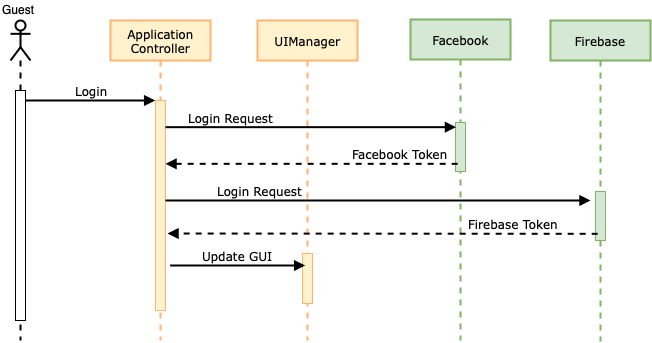
\includegraphics[width=1\textwidth]{images/Sequence/Login}
\end{figure}
\newpage

\subsection*{Logout}
La procedura di "Logout" inizia quando l'utente preme il relativo bottone del Side Menu. Una volta premuto verrà visualizzato un messaggio di conferma. In caso di approvazione verrà effettualo il logout da Facebook e Firebase.

Una volta completata questa procedura il sistema aggiornerà la GUI abilitando le sezioni non disponibili per i guest.

\begin{figure}[H]
	\centering
	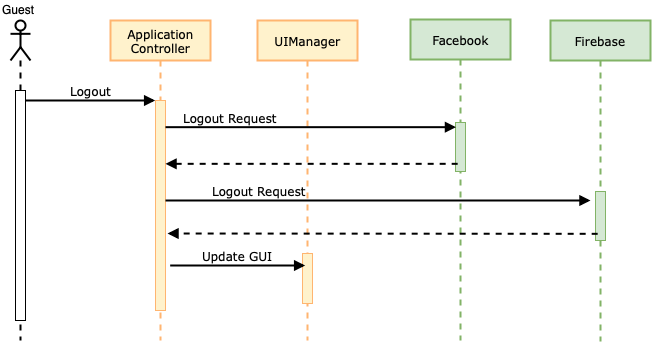
\includegraphics[width=1\textwidth]{images/Sequence/Logout}
\end{figure}
\newpage


\subsection*{View News}
The ”View News” procedure starts when the user opens the application or presses the ”News” section in the Tab Navigator. The sequence diagram shows the normal procedure.

After the user activates the News section, the application will send a request to the ”NewsAPI” service in order to obtain all the information related to the most important daily news.

Once this information is obtained, the Controller will create a UITableViewCell for each news and insert them into the TableView.

Furthermore and asynchronously, the application will download the preview images to allow the user to read the news headlines. When a cell is pressed the Controller will open a WebView addressed to the URL of the news in order to allow the user to read  the complete article.

\begin{figure}[H]
	\centering
	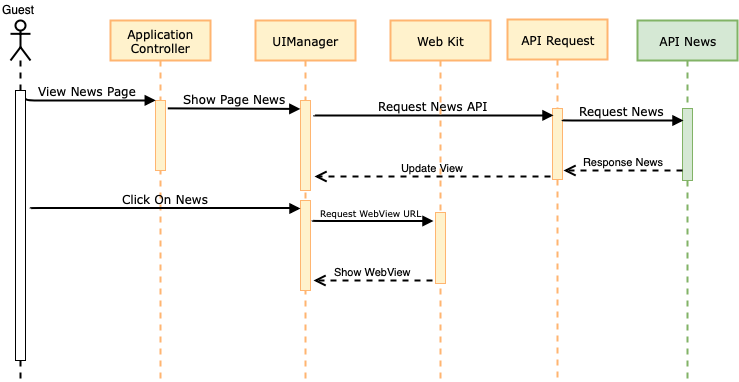
\includegraphics[width=1\textwidth]{images/Sequence/SequenceNews}
\end{figure}


\newpage

\subsection*{Share News}
The ”Share News” procedure starts when the user opens the application or presses the ”News” section in the Side Menu. The sequence diagram shows the normal procedure.

Dopo la normale procedura di "View News" l'utente preme sul bottone di share. A quel punto l'applicazione farà una richiesta alle "Graph" API di Facebook per la creazione del post con il testo inserito dall'utente.

Tale operazione ha come condizione che l'utente sia già autenticato e in caso contrario restituirà una avviso di errore.

\begin{figure}[H]
	\centering
	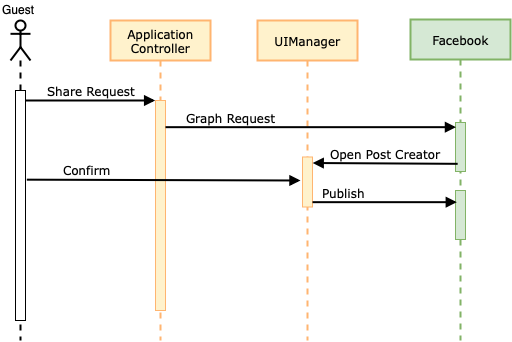
\includegraphics[width=1\textwidth]{images/Sequence/SharePost}
\end{figure}


\newpage



\subsection*{View Match}
The ”View Match” procedure starts when the user presses the “Live” section of the Tab Bar Navigator.

After activating the ”Live” section, the application will send a request to the ”API- Football” service to obtain information about the daily matches and their forecasts.

When this information has been reached, the Controller will create a UITableViewCell for all the matches and insert them into the TableView.

At regular intervals the Controller will repeat these requests to keep the matches updated.

\begin{figure}[H]
	\centering
	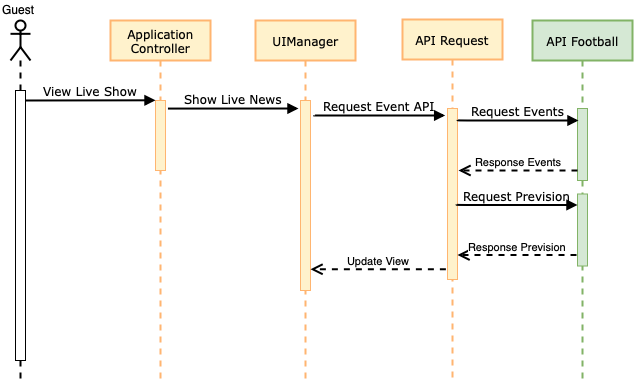
\includegraphics[width=1\textwidth]{images/Sequence/SequenceLive}
\end{figure}


\newpage
\subsection*{View Match Details}
The ”View Match” procedure starts when the user is in the ”Live” section and presses on a single match to know the details.

Now the Controller has access to the data for the specific match, previously downloaded from the “APIFootball” service and creates Views for every information. 

After opening the detail page, the user can change the desired information through the relative buttons.

\begin{figure}[H]
	\centering
	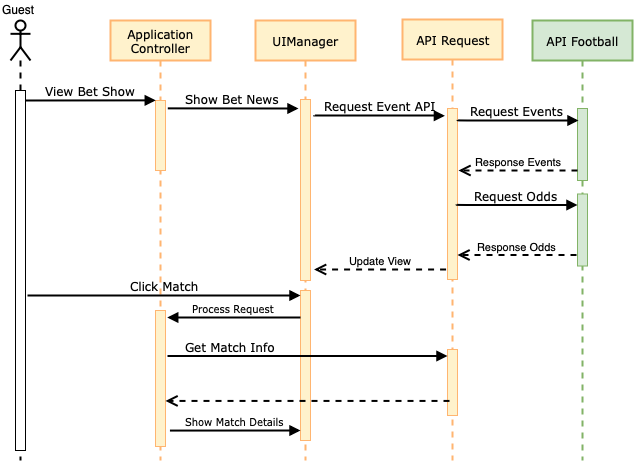
\includegraphics[width=1\textwidth]{images/Sequence/SequenceMatchDetails}
\end{figure}

\newpage

\subsection*{Chat}
La procedura di "Chat" inizia quando l'utente preme il relativo bottone del Side Menu. Una volta caricata la schermata, l'applicazione rimarrà in ascolto della room mostrando in tempo reale tutti i messaggi inviati dagli altri utenti. L'utente può poi scrivere e inviare il proprio messaggio.

L'applicazione inoltre scaricherà le immagini del profilo relative ai messaggi inviati dagli altri utenti in maniera asincrona.

Tale procedura presuppone che l'utente sia già autenticato altrimenti verrà visualizzato un messaggio di errore.

\begin{figure}[H]
	\centering
	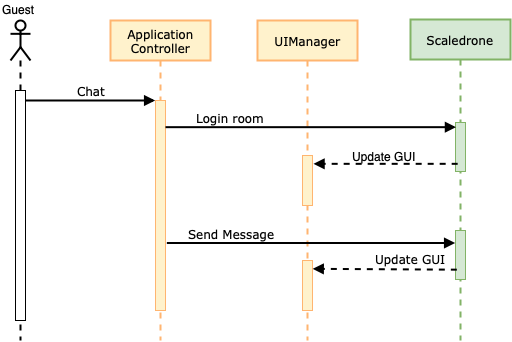
\includegraphics[width=1\textwidth]{images/Sequence/Chat}
\end{figure}
\newpage

\subsection*{View Odds}
The ”View Odds” procedure starts when the user presses the “Bet” section on the Tab Bar Navigator.

Activated the ”Bet” section, the application will send a request to the ”APIFootball” service to obtain information about the daily matches and the relative odds.

At this point, the Controller will create a UITableViewCell for each news and insert them into the TableView. In particular, we inserted three buttons (one for each prediction) with the relative odd indicated.

At regular intervals the Controller will repeat these requests to keep the matches updated.
\begin{figure}[H]
	\centering
	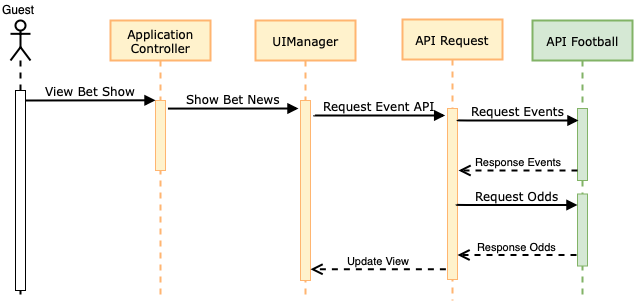
\includegraphics[width=1\textwidth]{images/Sequence/SequenceOdds}
\end{figure}

\newpage
\subsection*{Add Odd}
The ”Add Odd” procedure starts when the user is in the ”Bet” section and presses on  the prediction of the match he wants to bet on.

At that point the Controller has access to the data for the specific match, previously downloaded from the ”APIFootball” service and create the data structure that will be saved in the Database.

Once the data structure is created, the Controller will check if the match is already present in the database; If so, it will update the element with the new forecast, otherwise it will create a new record.

After updating the DB the Controller will update the current View to show the change in a visual feedback.

\begin{figure}[H]
	\centering
	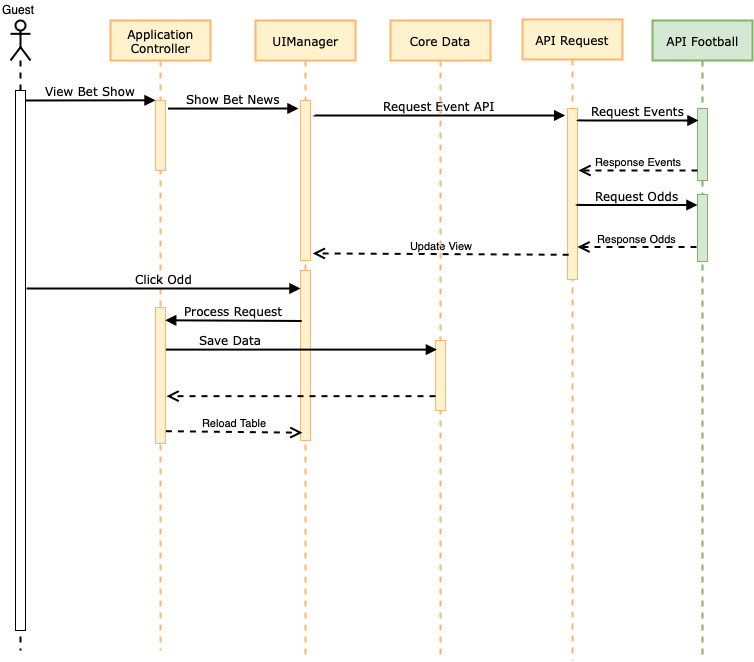
\includegraphics[width=1\textwidth]{images/Sequence/SequenceAddOdd}
\end{figure}
\newpage
\subsection*{View Cart}
The ”View Cart” procedure starts when the user is in the ”Bet” section and presses the button showing a cart in the Navigation bar.

At  that point, the Controller has access to the data in the Database and for each of them  it will create a UITableViewCell to be inserted in the TableView.

The user can change the amount of money gambled  by using the corresponding  input.  Once the amount has been updated, the Controller will calculate the potential winnings by multiplying all the odds with the amount played.

\begin{figure}[H]
	\centering
	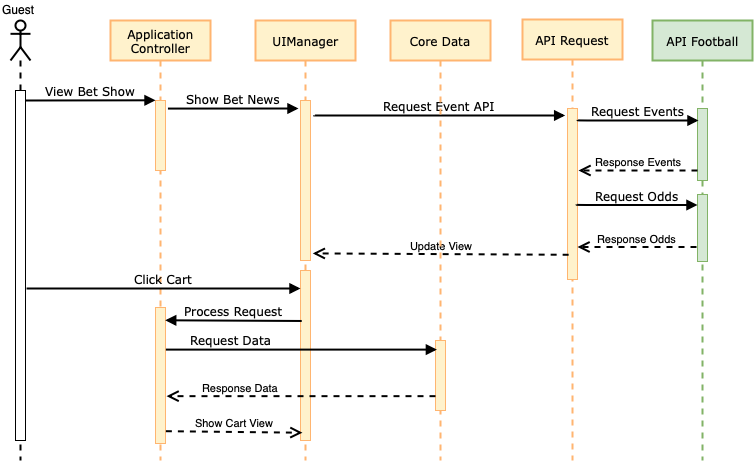
\includegraphics[width=1\textwidth]{images/Sequence/SequenceViewCart}
\end{figure}
\newpage
\subsection*{Remove Odd}
The procedure of  ”Remove Odd” begins when the user is in the ”Bet” section and he is checking the cart.

In this section the user can delete each bet by swiping to the left with his finger.

At that point the Controller will delete the corresponding record from the Database and update the contents of the shopping cart also recalculating the new potential winnings.
\begin{figure}[H]
	\centering
	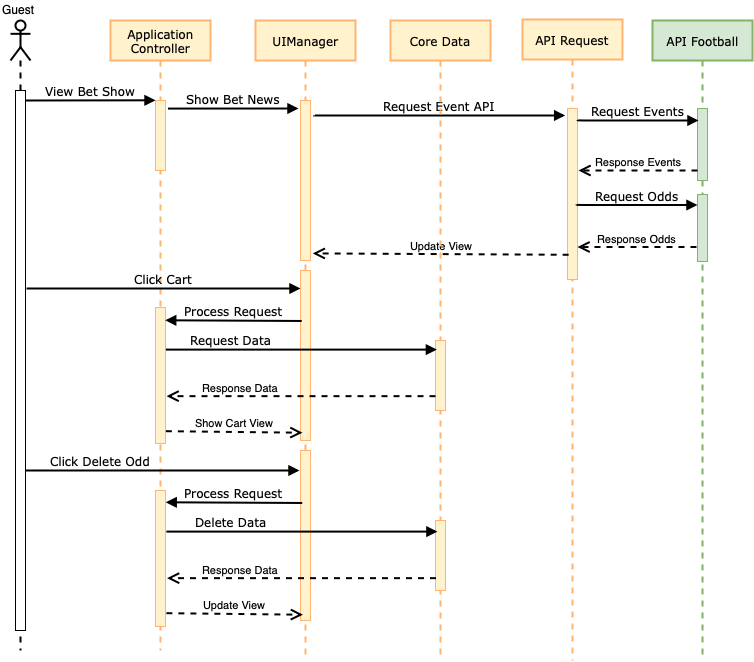
\includegraphics[width=1\textwidth]{images/Sequence/SequenceRemoveOdd}
\end{figure}

\newpage

\subsection*{Buy Ticket}

La procedura di "Buy Ticket" inizia dopo che l'utente ha completato la composizione della propria schedina.

Una volta premuto il bottone di buy l'applicazione controllerà la correttezza della schedina ed effettuerà l'acquisto 

Tale procedura presuppone che l'utente sia già autenticato altrimenti verrà visualizzato un messaggio di errore.

\begin{figure}[H]
	\centering
	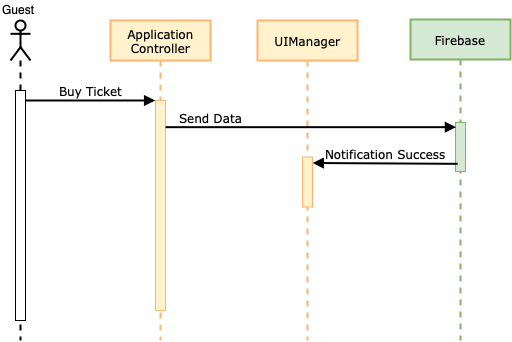
\includegraphics[width=1\textwidth]{images/Sequence/BuyTicket}
\end{figure}

\newpage

\subsection*{Ticket Chronology}
La procedura di "Ticket Chronology" inizia quando l'utente si trova nella sezione "Bet" dopo aver premuto il relativo bottone del Side Menu.

Dopo che l'utente preme sul tasto "Cronologia" del NavBar l'applicazione accederà ai dati presenti nel database di Firebase recuperando tutte le schedine acquistate in precedenza dall'utente e mostrandole a schermo

Tale procedura presuppone che l'utente sia già autenticato altrimenti verrà visualizzato un messaggio di errore.
\begin{figure}[H]
	\centering
	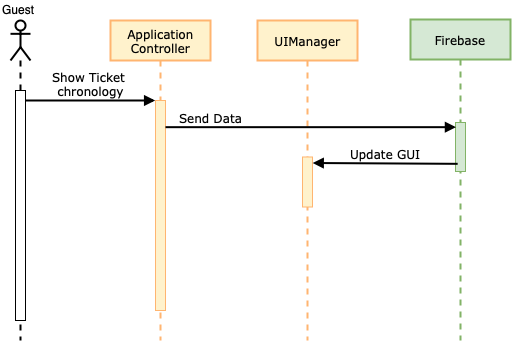
\includegraphics[width=1\textwidth]{images/Sequence/TicketChronology}
\end{figure}


\chapter{User Interfaces}
\chapter{External Services and Libraries}
iSport application uses several third parties API in order to provide all the services to the user.\\
Per il parsing dei dati JSON è stato usato il componente JSONDecoder nativo dell UIKit.
\subsection*{NewsAPI}
Quando un utente vuole visualizzare le principali notizie del giorno l'applicazione esegue le seguenti operazioni:
\begin{itemize}
	\item Esegue una richiesta GET al l'endpoint fornito dal servizio
	\item Se la risposta è valida effettua il parsing del contenuto JSON
	\item Crea le celle della tabella contenente le informazioni fornite dal servizio e parsate
	\item Scarica in maniera asincrona le immagini di anteprima
\end{itemize}
L'endpoint utilizzato è "https://newsapi.org/v2/top-headlines?country=it\&category=sports \&apiKey=API\_KEY". La risposta fornita dal servizio è:
\begin{figure}[H]
	\centering
	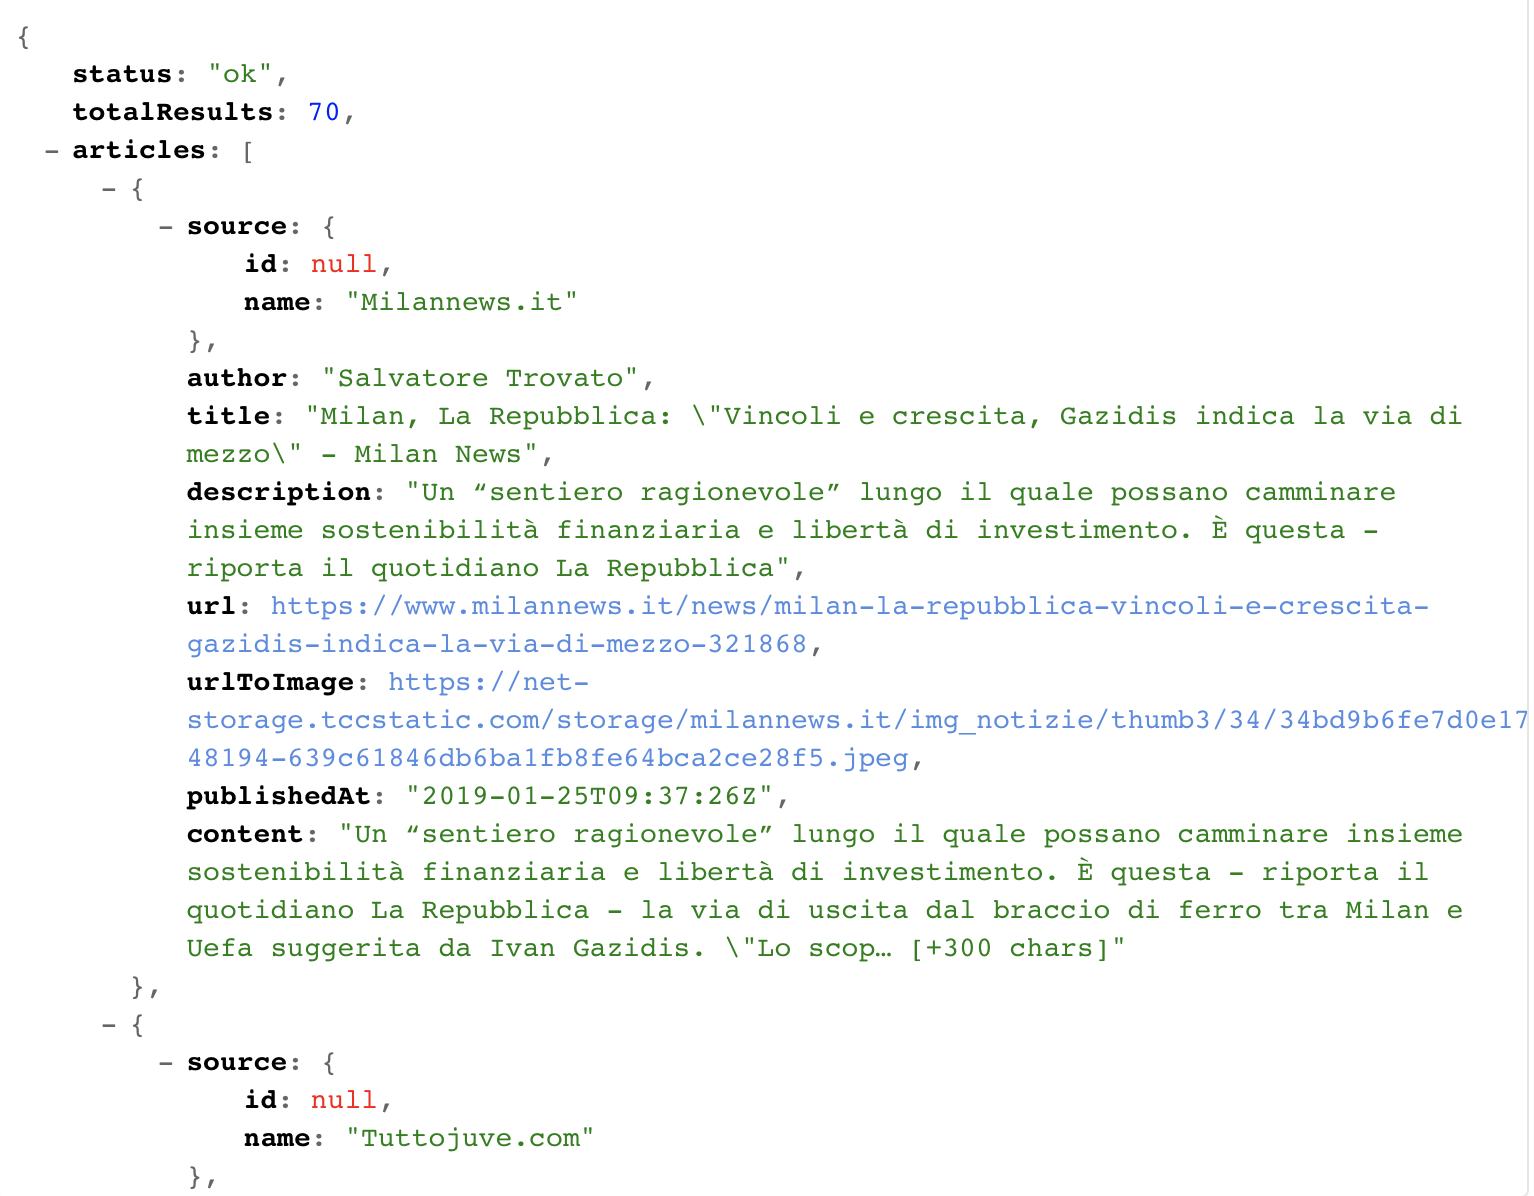
\includegraphics[width=0.7\textwidth]{images/ResponseNewsAPI}
\end{figure}
Per il parsing quindi è stata usata la seguente struttura dati:
\begin{figure}[H]
	\centering
	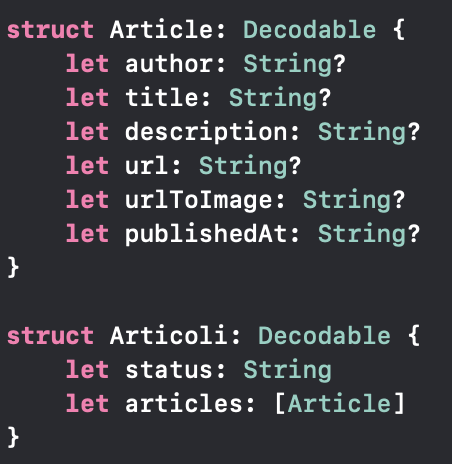
\includegraphics[width=0.3\textwidth]{images/StructDati}
\end{figure}
\subsection*{APIFootball}
Quando un utente vuole visualizzare i risultati delle partite del giorno l'applicazione esegue le seguenti operazioni:
\begin{itemize}
	\item Esegue una richiesta GET al l'endpoint fornito dal servizio
	\item Se la risposta è valida effettua il parsing del contenuto JSON
	\item Crea le celle della tabella contenente le informazioni fornite dal servizio e parsate
	\item Aggiorna le informazioni ogni 30 secondi per mantenere i dati in tempo reale
\end{itemize}
L'endpoint utilizzato per ottenere i risultati è "https://apifootball.com/api/?action=get\_events". La risposta fornita dal servizio è:
\begin{figure}[H]
	\centering
	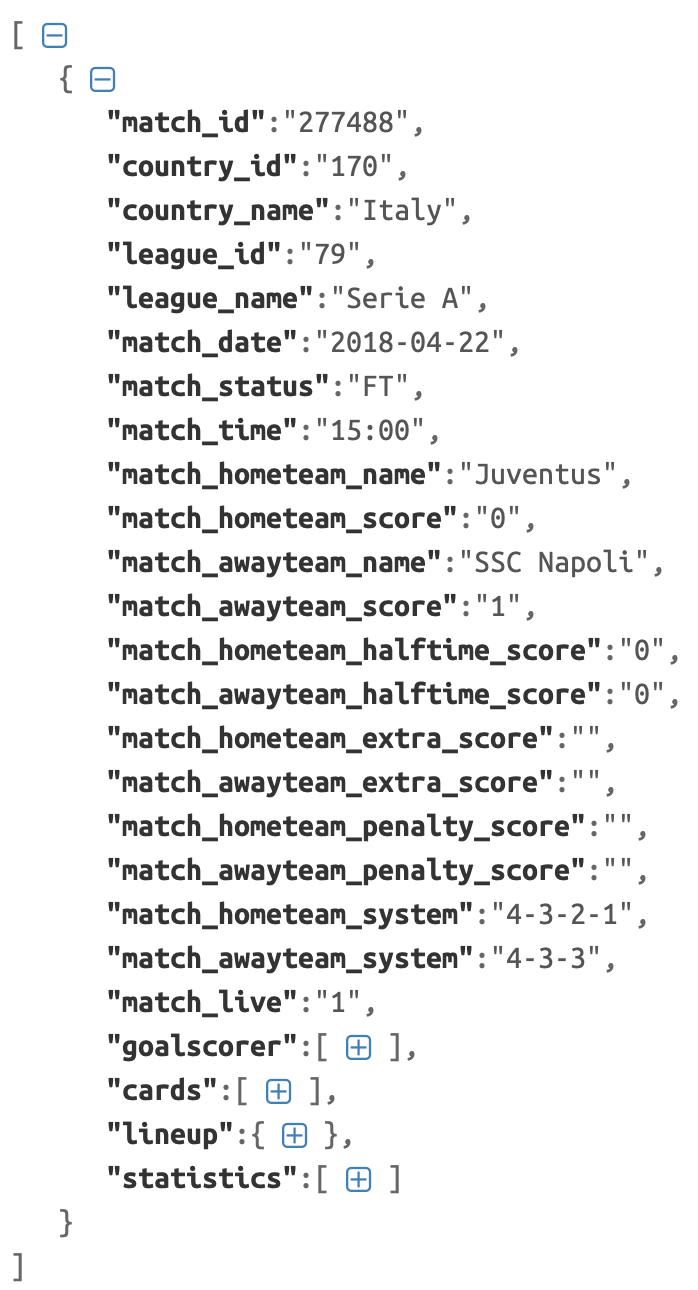
\includegraphics[width=0.3\textwidth]{images/ResponseCompleta}
\end{figure}
Per il parsing quindi è stata usata la seguente struttura dati:
\begin{figure}[H]
	\centering
	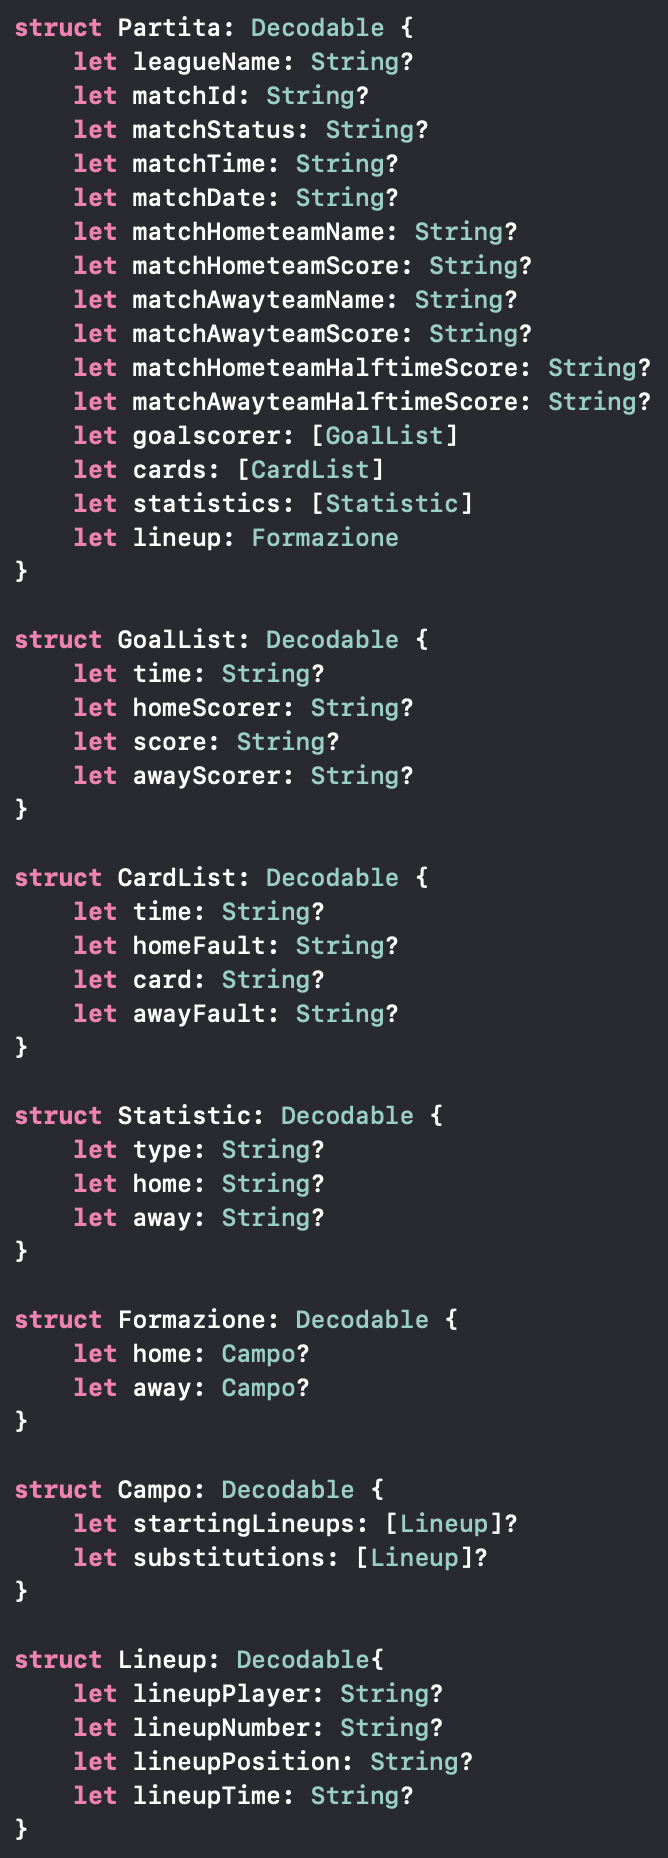
\includegraphics[width=0.3\textwidth]{images/StructPartita}
\end{figure}
Per ottenere le previsioni della partita l'endpoint utilizzato è "https://apifootball.com/api/? action=get\_predictions". La risposta fornita dal servizio è:
\begin{figure}[H]
	\centering
	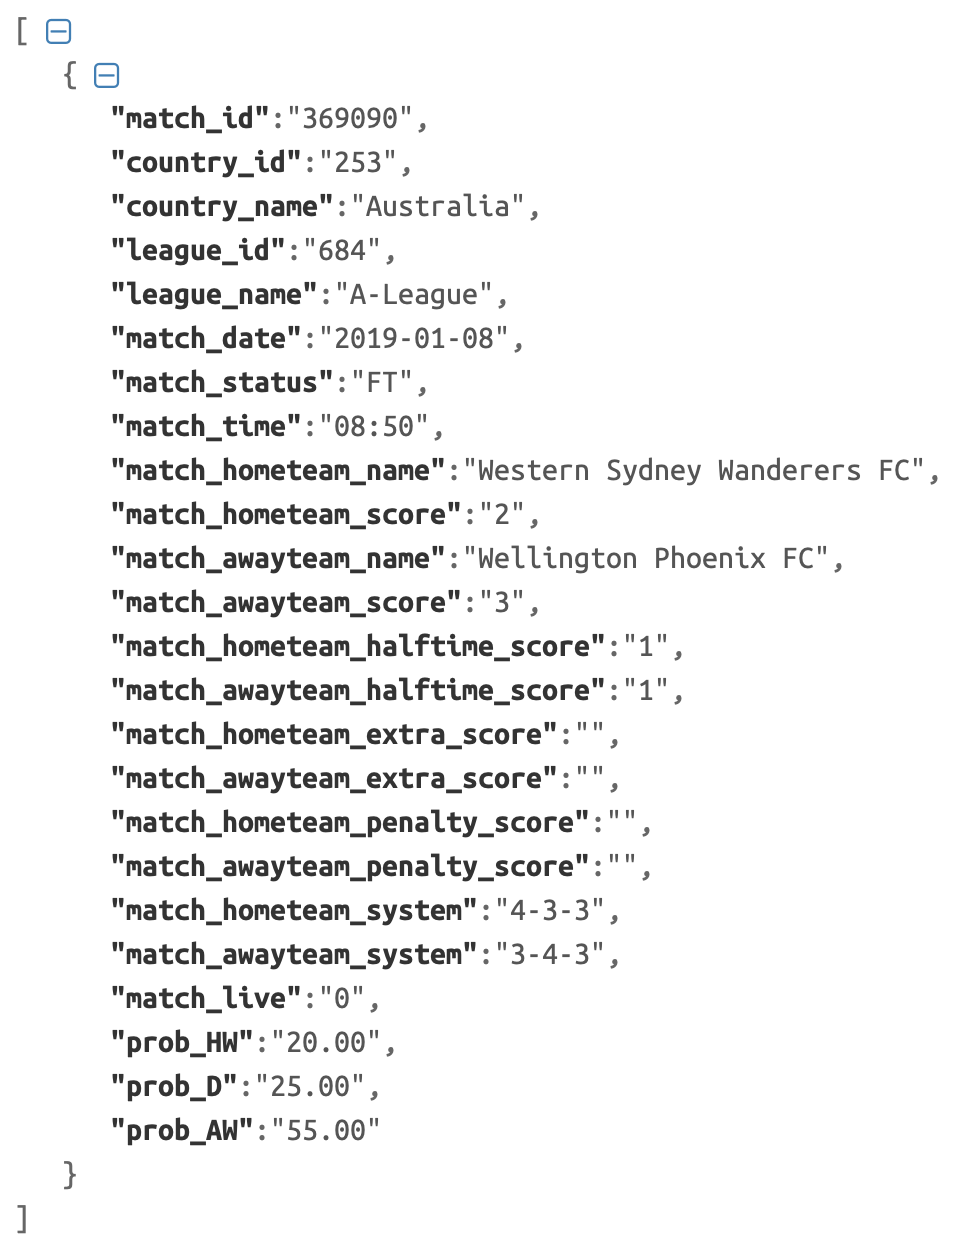
\includegraphics[width=0.3\textwidth]{images/ResponsePrediction}
\end{figure}
Per il parsing quindi è stata usata la seguente struttura dati:
\begin{figure}[H]
	\centering
	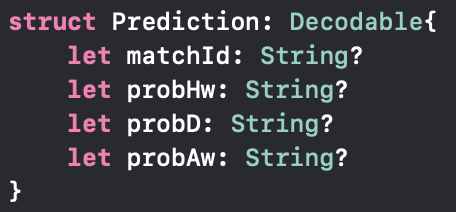
\includegraphics[width=0.3\textwidth]{images/StructPrediction}
\end{figure}
Per ottenere le quote delle partite l'endpoint utilizzato è "https://apifootball.com/api/? action=get\_odds". La risposta fornita dal servizio è:
\begin{figure}[H]
	\centering
	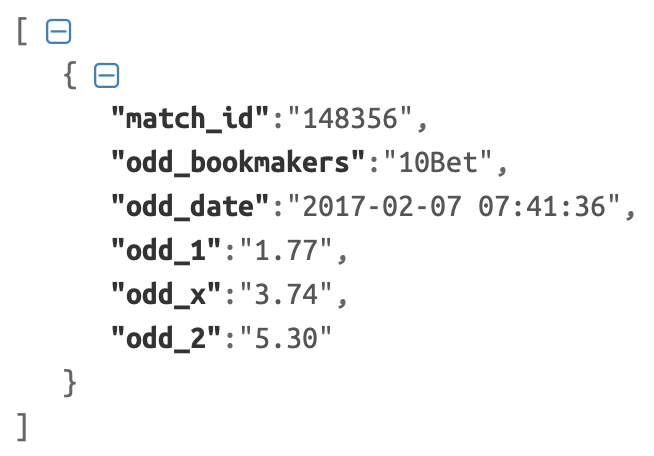
\includegraphics[width=0.3\textwidth]{images/ResponseOdds}
\end{figure}
Per il parsing quindi è stata usata la seguente struttura dati:
\begin{figure}[H]
	\centering
	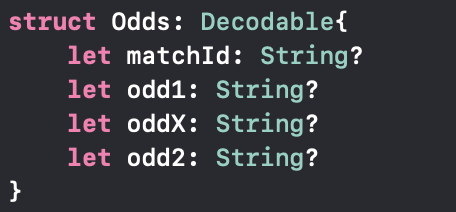
\includegraphics[width=0.3\textwidth]{images/StructOdds}
\end{figure}


\chapter{Software System Attribute}
\section{Reliability}
As the majority of function requires an internet connection, the software is reliable as long as there are no connectivity problems.
\section{Availability}
The availability parameter also relies on the internet connection signal and on the responses provided by "https://newsapi.org" and "https://apifootball.com". No problems of availability were found both during the developement phase and beta testing with users.
\section{Security}
The security of the iSport application was the main concern during the developement. As all the information provided are retrived from the web, there are different checks to perform in order to keep the user information safe. Furthermore, for the communication with external services, was chosen HTTPS protocol to guarantee greater security
\section{Maintainability}
The entire application is very maintainable as the code is entirely documented, in particular in several critical function. Therefore any developer who wants to improve it or make changes is able to do it without relevant difficulty.
\section{Usability}
The usability was another of our concern for the development. In order to improve it, a beta version of the application was given to 5 users and tested for 1 weeks. The result of this test highlighted usability issues. In particular, in the first version the buttons for changing information on the match detail page were not clearly visible. Another report concerned the lack of visual feedback after adding a quota to their ticket. Both of these problems were then solved in a later version of the application.

\chapter{Test Cases}
\chapter{Cost Estimation}







\end{document}
